\section{Galilean Transformations and Lorentz Transformations}

\instructornote{%
By Matt Trawick, 2019.  Time: 40 minutes

This lab doesn't do much in the way of 

Activity 1 assumes that students have already seen the idea of time dilation and the Lorentz factor $\gamma$, probably by analyzing this exact situation with Anna, Bob, a train, and a flashlight, as in a previous lab.

Activity 2 assumes that students have been introduced to the idea that simultaneity is relative, again, probably by having seen this exact same situation of Anna on a train with two lightbulbs.

Someday Matt might write an Activity 3 that would focus on the difference between proper distance and proper length.
}

\makelabheader %(Space for student name, etc., defined in master.tex or labmanual_formatting_commands.tex)

\bigskip
\textbf{Apparatus:}
\begin{itemize}[nosep]
\item \textit{Mathematica}, with notebook file \filename{minkowski\_events.nb}
\end{itemize}


\bigskip


\textbf{Activity 1: Transformations in Space and Time}

You have previously discussed a thought experiment in which Anna rides a train at speed $v$.  She aims a laser beam at a mirror on the floor of the train, and measures the time $\Delta t_0$ that it takes from the time the photon is 
\begin{wrapfigure}[4]{r}{0.35\textwidth}
\begin{center}
\vspace{-0.3in}
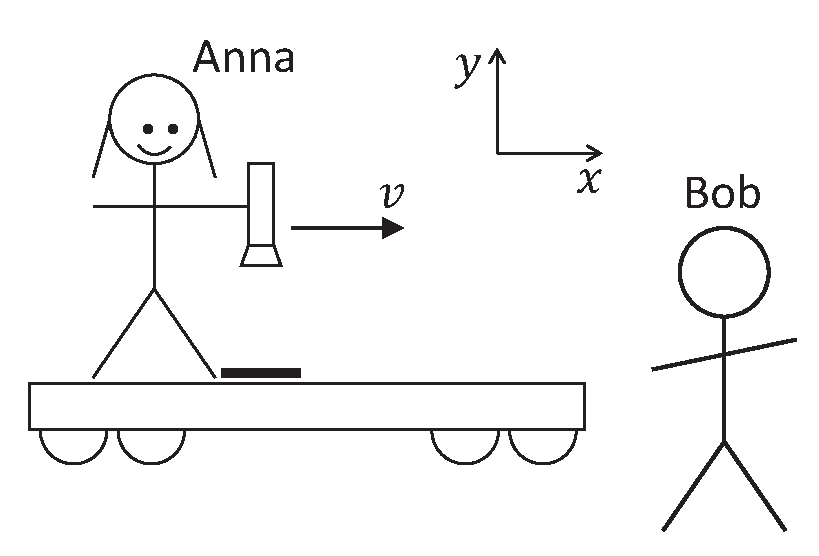
\includegraphics[scale=0.4]{lorentz_transformations/anna_and_bob.eps}
\end{center}
\end{wrapfigure}
emitted to when the photon returns to the laser.  Bob observes the same experiment, standing near the tracks beside the train.  

\begin{enumerate}[labparts]

\item  
On the axes below on the left, draw a spacetime graph (Minkowski diagram) of these two events as seen in Anna's reference frame, taking the emission of the photon to happen at $x=0$ and $t=0$.
\end{enumerate}

\vspace{0.2in}

\begin{center}
%\raisebox{0.7in}{\parbox{1in}{Galilean \newline Transformation:}}\hspace{0.2in}
\begin{lab_axis}[lab_noticks_4quads,
	width=1.5in, height=1.5in,
	xlabel={$x$},
	ylabel={$t$},
	title style={at={(0.5,1)}},
	title={Anna's Frame}
	]
\addplot +[dashed, thin, gray] {x};
\addplot +[dashed, thin, gray] {-x};
\end{lab_axis}
\hspace{0.2in}
\raisebox{0.72in}{$\xleftrightarrow[\mbox{Transformation}]{\mbox{Galilean}}$}
\hspace{0.2in}
\begin{lab_axis}[lab_noticks_4quads,
	width=1.5in, height=1.5in,
	xlabel={$x'$},
	ylabel={$t'$},
	title style={at={(0.5,1)}},
	title={Bob's Frame}
	]
\addplot +[dashed, thin, gray] {x};
\addplot +[dashed, thin, gray] {-x};
\end{lab_axis}
\end{center}
\begin{enumerate}[labparts,resume]

\item 
Now consider the same two events in the reference frame of Bob, who is standing beside the tracks so that the emission of the photon  happens at $x'=0$ and $t'=0$ in his reference frame too.
On the axes above on the right, draw a spacetime graph of these two events as seen in Bob's reference frame, according to the principle of Galilean relativity (as described the Galilean transformations).

\item Once you have drawn your graph, you can check your answer by 
opening the file \filename{minkowski\_events.nb}, which will open in Mathematica.  Type \button{Ctrl-A} to select everything, and type \button{Shift-Enter} to excute all of the lines you have selected.  Then scroll down to the first graph you see, titled ``Galilean Transformation''.  You can see the line of code above the graph that generates the two points at (5,1) and (3,2). Edit the locations of those points to the values for the two events in Anna's reference frame, and hit \button{Shift-Enter} to excute your changes.  Use the slider to see the events in Bob's reference frame, and make any corrections needed on your graphs above.

\item The graph you drew for Bob's reference frame is inconsistent with the principle of relativity, because it implies that the speed of light is not the same in all reference frames.  In Anna's frame, light travels only the vertical distance down and back in some time $t$.  In Bob's frame, the light travels a longer, diagonal path.  According to the Galilean transformations, it does so in the same time $t$ as in Anna's frame, which would mean that Bob would see the light going faster than Anna does.  To correct this, would the time $t$ of the light returning to the flashlight be \textit{earlier} or \textit{later} than in Anna's frame?
\answerspace{0.4in}

\pagebreak[2]
\item On the axes below, redraw the two events as seen in Anna's reference frame on the axes to the left.  On the axes on the right, draw the two events as you know they should be, consistent with the principle of relativity.

\begin{center}
%\raisebox{0.7in}{\parbox{1in}{Lorentz \newline Transformation:}}\hspace{0.2in}
\begin{lab_axis}[lab_noticks_4quads,
	width=1.5in, height=1.5in,
	xlabel={$x$},
	ylabel={$t$},
	title style={at={(0.5,1)}},
	title={Anna's Frame}
	]
\addplot +[dashed, thin, gray] {x};
\addplot +[dashed, thin, gray] {-x};
\end{lab_axis}
\hspace{0.2in}
\raisebox{0.72in}{$\xleftrightarrow[\mbox{Transformation}]{\mbox{Lorentz}}$}
\hspace{0.2in}
\begin{lab_axis}[lab_noticks_4quads,
	width=1.5in, height=1.5in,
	xlabel={$x'$},
	ylabel={$t'$},
	title style={at={(0.5,1)}},
	title={Bob's Frame}
	]
\addplot +[dashed, thin, gray] {x};
\addplot +[dashed, thin, gray] {-x};
\end{lab_axis}
\end{center}

  

\item Now that you have drawn your graph above, you can check your answers again using the same Mathematica simulation as before, but this time scroll down further to the second graph, titled "Lorentz Transformation''.  Again, edit the positions of the two green points, and move the slider to represent the speed of Bob's reference frame relative to Anna's.  Was your prediction correct?  Note any corrections on the graphs above, as needed. 

\medskip
Galilean transformations just don't account for relativistic effects like time dilation or length contraction at very high speeds, though they are an excellent approximation at low speeds, $v \ll c$.  The second graph in the Mathematica file uses \textit{Lorentz transformations} instead, which properly account for changes in space and time at high speeds. 
\end{enumerate}

\textbf{Activity 2: Simultaneity and the Speed of Light}

Anna rides on a train in the $+x$ direction.  Facing the side of a train car, she holds out her arms (each one meter long) to the sides, with one lightbulb in each hand.  In Anna's reference frame, the bulbs turn on simultaneously.  Bob views this while standing beside the tracks as the train zooms by.

\begin{enumerate}[labparts]
\item On the axes below on the left, draw a spacetime diagram in the reference frame of Anna showing three events: each of the two lightbulbs turning on, and the photons from both bulbs arriving at the tip of Anna's nose.  Take the photons arriving at Anna's nose to happen at $x=0$ and $t=0$.  On the axes to the right, draw the same three events as they would occur in Bob's reference frame, moving to the left with velocity $v=-0.5c$, \textit{according to the Galilean transformations.}

\begin{center}
%\raisebox{0.7in}{\parbox{1in}{Galilean \newline Transformation:}}\hspace{0.2in}
\begin{lab_axis}[lab_noticks_4quads,
	width=1.5in, height=1.5in,
	xlabel={$x$},
	ylabel={$t$},
	title style={at={(0.5,1)}},
	title={Anna's Frame}
	]
\addplot +[dashed, thin, gray] {x};
\addplot +[dashed, thin, gray] {-x};
\end{lab_axis}
\hspace{0.2in}
\raisebox{0.72in}{$\xleftrightarrow[\mbox{Transformation}]{\mbox{Galilean}}$}
\hspace{0.2in}
\begin{lab_axis}[lab_noticks_4quads,
	width=1.5in, height=1.5in,
	xlabel={$x'$},
	ylabel={$t'$},
	title style={at={(0.5,1)}},
	title={Bob's Frame}
	]
\addplot +[dashed, thin, gray] {x};
\addplot +[dashed, thin, gray] {-x};
\end{lab_axis}
\end{center}

\item As before, check your results using the \textit{Galilean Transformation} simulation in Mathematica, noting any corrections on your axes above.  Was your initial graph correct?
\answerspace{0.4in}

\item Are the two graphs above consistent with the principle of relativity?  Why or why not?
\answerspace{0.6in}

\pagebreak[2]
\item On the axes below, redraw the same three events in both Anna's reference frame and Bob's reference frame, according to the Lorentz transformation.  You can try it on your own first if you like, then use the Lorentz Transformation simulation in Mathematica to confirm or correct your understanding.

\begin{center}
%\raisebox{0.7in}{\parbox{1in}{Lorentz \newline Transformation:}}\hspace{0.2in}
\begin{lab_axis}[lab_noticks_4quads,
	width=1.5in, height=1.5in,
	xlabel={$x$},
	ylabel={$t$},
	title style={at={(0.5,1)}},
	title={Anna's Frame}
	]
\addplot +[dashed, thin, gray] {x};
\addplot +[dashed, thin, gray] {-x};
\end{lab_axis}
\hspace{0.2in}
\raisebox{0.72in}{$\xleftrightarrow[\mbox{Transformation}]{\mbox{Lorentz}}$}
\hspace{0.2in}\begin{lab_axis}[lab_noticks_4quads,
	width=1.5in, height=1.5in,
	xlabel={$x'$},
	ylabel={$t'$},
	title style={at={(0.5,1)}},
	title={Bob's Frame}
	]
\addplot +[dashed, thin, gray] {x};
\addplot +[dashed, thin, gray] {-x};
\end{lab_axis}
\end{center}

\item In the graphs above, is light traveling at speed $c$ in both reference frames?
\answerspace{0.6in}

\item Are the two events of the bulbs turning on simultaneous in both reference frames?


\end{enumerate}
